\documentclass[11.5pt]{sig-alternate} % sets document style to sig-alternate
% packages
% typesetting
%\usepackage{dirtytalk} % typset quotations easier (\say{stuff})
\usepackage{hanging} % hanging paragraphs
\usepackage[defaultlines=3,all]{nowidow} % avoid widows
\usepackage[pdfpagelabels=false]{hyperref} % produce hypertext links, includes backref and nameref
\usepackage{xurl} % defines url linebreaks, loads url package
\usepackage{microtype}
%\usepackage[super]{nth} % easily create superscript ordinal numbers with \nth{x}
\usepackage{textcomp}
\newcommand{\texttildemid}{\raisebox{0.4ex}{\texttildelow}}
% layout
%\usepackage{enumitem} % control layout of itemize, enumerate, description
\usepackage{fancyhdr} % control page headers and footers
\usepackage{float} % improved interface for floating objects
%\usepackage{multicol} % intermix single and multiple column pages
% language
\usepackage[utf8]{inputenc} % accept different input encodings
\usepackage[english]{babel} % multilanguage support
% misc
\usepackage{graphicx} % builds upon graphics package, \includegraphics
%\usepackage{lastpage} % reference number of pages
%\usepackage{comment} % exclude portions of text (?)
\usepackage{xcolor} % color extensions
\usepackage[backend=biber, style=apa]{biblatex} % sophisticated bibliographies % necessary for HTML to display author info and date on abstract page
\usepackage{csquotes} % advanced quotations, makes biblatex happy
\usepackage{authblk} % support for footnote style author/affiliation
% tables and figures
\usepackage{tabularray}
%\usepackage{array} % extend array and tabular environments
\usepackage{caption} % customize captions in figures and tables (rotating captions, sideways captions, etc)
%\usepackage{cuted} % allow mixing of \onecolumn and \twocolumn on same page
\usepackage{multirow} % create tabular cells spanning multiple rows
%\usepackage{subfigure} % deprecated, support for manipulation of small figures
%\usepackage{tabularx} % extension of tabular with column designator "x", creates paragraph-like column whose width automatically expands
%\usepackage{wrapfig} % allows figures or tables to have text wrapped around them
%\usepackage{booktabs} % better rules
% dummy text
%\usepackage{blindtext} % blind text dummy text
%\usepackage{kantlipsum} % Kant style dummy text
\usepackage{lipsum} %lorem ipsum dummy text
% other helpful packages may be booktabs, longtable, longtabu, microtype

\pagestyle{fancy} % sets pagestyle to fancy for fancy headers and footers

% header and footer
% modern way to set header image
\renewcommand{\headrulewidth}{0pt} % defines thickness of line under header
\renewcommand{\footrulewidth}{0pt} % defines thickness of line above header
\setlength\headheight{80.0pt} % sets height between top margin and header image, effectively moves page contents down
\addtolength{\textheight}{-80.0pt} % seems to affect the lower height. maybe only works properly if footer numbers enabled?
\fancyhf{}
\fancyhead[CE, CO]{
\includegraphics[width=\textwidth]{headerImage.png}}
% footer
%\fancyfoot[LE,LO]{Article Title Here \\ DOI: }% left footer article title and doi
%\fancyfoot[CE,CO]{{}} % center footer empty
%\fancyfoot[RE,RO]{\thepage} % right footer page numbers
%\pagenumbering{arabic} % arabic (1, 2, 3) numbering in footer

\hypersetup{colorlinks=true,urlcolor=blue} % sets link color to blue
\urlstyle{same} % sets url typeface to same as rest of text

% set caption and figure to italics, label bold, left align captions, does not transfer to HTML
\captionsetup{labelfont=bf, font={large, it}, justification=raggedright, singlelinecheck=false}
\renewcommand\theContinuedFloat{\alph{ContinuedFloat}}

%this next bit is confusing, but essentially changes the width of the abstract. Seems to have been copied from this https://tex.stackexchange.com/questions/151583/how-to-adjust-the-width-of-abstract
\let\oldabstract\abstract
\let\oldendabstract\endabstract
\makeatletter %changes @ catcode to enable modification (in parsep)
\renewenvironment{abstract} %alters the abstract environment
{\renewenvironment{quotation}%
               {\list{}{\addtolength{\leftmargin}{1em} % change this value to add or remove length to the the default ?
                        \listparindent 1.5em%
                        \itemindent    \listparindent%
                        \rightmargin   \leftmargin%
                        \parsep        \z@ \@plus\p@}%
                \item\relax}%
               {\endlist}%
\oldabstract}
{\oldendabstract}
\makeatother %changes @ catcode to disable modification

% checks
% italics -
% links -
% dashes -
% tildes -
\begin{document}

\title{Assessment of Climate Science Knowledge and Perceptions of Deaf and Hard-of-Hearing Students}

\author[1]{\large \color{blue}Annemarie D. Ross}
\author[1]{\large \color{blue}Kyle Edenzon}
\author[2]{\large \color{blue}Susan Smith Pagano}
\author[3]{\large \color{blue}Randy Yerrick}
\author[1]{\large \color{blue}Todd Pagano}

\affil[1]{Department of Science and Mathematics, National Technical Institute for the Deaf Rochester Institute of Technology}
\affil[2]{Thomas H. Gosnell School of Life Sciences Rochester Institute of Technology}
\affil[3]{Department of Learning and Instruction, The State University of New York at Buffalo}

\toappear{}
%% ABSTRACT
\maketitle
\begin{@twocolumnfalse} 
\begin{abstract}
\item 
\textit{Curricula related to sustainability and climate science are being integrated into academic science courses and programs.  We set out to assess the knowledge of some of these environmental concepts among a group of Deaf/Hard-of-Hearing (D/d/HH) postsecondary students.  A survey that attempted to gauge student understanding and perceptions of climate science was developed, administered to D/d/HH and hearing college students, and analyzed.  Preliminary results showed that there could be some gaps in related knowledge among the D/d/HH group.  Rasch analysis was then used to assess the quality of the survey for the intended outcomes and improved iterations of the survey were developed and further evaluated for use with D/d/HH students.  Through this work, we found that it is important to examine the language contained in the designed instrument in order to assess the true understanding of D/d/HH students (and most likely, other English Language Learners).  This study could inform the development of interventions and curricular changes for D/d/HH students related to climate science topics.}
\\ \\ 
\end{abstract}
\end{@twocolumnfalse}

%% AUTHOR INFORMATION

\textbf{*Corresponding Author, Annemarie D. Ross}\\
\href{mailto:  adrnts@rit.edu}{ (adrnts@rit.edu)} \\
\textit{Submitted  February 15, 2019}\\
\textit{Accepted July 14, 2019} \\
\textit{Published online July 29, 2019} \\
\textit{DOI: 10.14448/jsesd.11.0009} \\
\pagebreak
\clearpage
\begin{large}

\section*{INTRODUCTION}

A current trend in higher education is to integrate concepts of sustainability, systems-thinking, and operating “green” into the curriculum and campus functions.  One goal of this movement is to educate the general student to be an environ\-ment-literate citizen, while another is to train future scientists to incorporate “green thinking”, like attention to life cycle analysis, into their experimental designs. An understanding of climate science topics is central to this way of thinking as the production, transportation, use, and disposal of products and consumables negatively impacts the climate (largely via the accumulation of carbon dioxide).  Therefore, there is a real need for applying environmental sustainability issues, and climate science concepts, to the student educational experience.

Though we have begun to see examples of sustainability (Timmer et al., 2018), life cycle assessment (Guron, Paul, \& Roeder, 2016), and climate science (Chang, Pascua, \& Ess, 2018) in the science education curriculum, not much attention has been given to implementing these topics into curricula for students with disabilities, and particularly, Deaf and Hard-of-Hearing (D/d/HH) students. Interventions targeting students in the traditional classroom often do not work in the D/d/HH classroom (Ross, Yerrick, \& Pagano, 2019b). On a side note, we chose the abbreviation ‘D/d/HH’ to respect Deaf culture and follow form that within the culture “identity-first” (as opposed to “people-first”) language is often preferred. While records related to the education of the D/d/HH community are well documented and go back to the 1800’s, there is little research or evidence of how D/d/HH students respond to current curricular or pedagogical methods for teaching environmental concepts. Before developing strategies to teach these concepts, it is important to assess the current level of understanding that D/d/HH students might have on related topics, as well as their perceptions as to how they feel they can perform as cognizant members of society related to these issues.

We developed a survey to assess the knowledge and perceptions of D/d/HH students on climate science/ climate change concepts and compared their results to a group of their hearing peers.  We further assessed the performance of the survey (via Rasch analysis) to determine if our instrument was indeed measuring the knowledge that we intended.  This analysis led to further iterations and refinement of the survey for use with D/d/HH students.  Related to this study, we developed a curricular intervention for the teaching of climate science concepts to D/d/HH students (Ross, Yerrick, \& Pagano, 2019a; Ross et al., 2019b). 

\subsection*{Educational Interventions for D/d/HH Students}

It is well-known that communication, in the sense of the mode of information transfer from one individual to another (i.e. auditory, visual, etc.), is a key component of the educational process.  Instructors often lecture and hearing students can hear the lectures and (hopefully) retain the information.  D/d/HH students do not always have access to this kind of direct communication as their hearing peers (Siegel, 2000). D/d/HH students often rely on other modes, like through an interpreter or open-caption devices. As a result, D/d/HH students can miss critical pieces of information if the teaching and communication are not conducive to their learning and communication needs. For example, D/d/HH students can miss out on incidental learning opportunities instances where individuals pick up knowledge from indirect/side conversations (perhaps between the instructor and one subgroup of students in the class). Such missed opportunities prevent information from reaching D/d/HH students (Hopper, 2011; King, 2017). 

Studies have compared educational performance between D/d/HH and hearing students (Gertz \& Boudreault, 2016; Marschark, 2001, 2011); however, there is very little, if any, research that shows the gap specifically tied to environmental education. One project that was developed in an attempt to find another method of educating D/d/HH students within the field of climate science was a web-based instruction system (Saksiri \& Suphajanya, 2010). The method involved the use of 3D characters signing, in American Sign Language (ASL), as the main mode of communication. Their research showed that 75\% of participants agreed that the climate science web-based instruction was easy to learn and efficient to use (Saksiri \& Suphajanya, 2010), but detailed statistics and comparisons to the performance of hearing peers were not given as part of the study. 

Overall, the lack of information available related to the teaching of environmental sustainability issues (and particularly as it relates to climate science) for D/d/HH students, in combination with issues related to communication access for D/d/HH students, might create a gap in the understanding of environmental/sustainability topics among students.  If such gaps exist, interventions could be established to remedy lack of understanding (or prevalence of misunderstandings) and improve the educational experience for D/d/HH students.  

\section*{PROJECT DESCRIPTION}

A survey was developed to help determine if gaps in the understanding of sustainability and climate science issues among a group of D/d/HH students exists.  This instrument also attempted to gain insights into students’ levels of perceived confidence with these concepts and the amount of coursework that they have taken with environmental content.  In total, 80 students at Rochester Institute of Technology (RIT, Rochester, NY) and the National Technical Institute for the Deaf (NTID, a college of RIT) anonymously completed the initial version of the survey.  For consistency, only students who were science majors completed the survey.  Coincidently, of the 80 students who took the survey, 40 were D/d/HH and 40 forty were hearing. We did not predict that the participants’ demographics would be so evenly balanced in this regard, nor was this exact balance sought in our experimental design.  Other indicators (number of courses with environmental content previously taken, type of high school attended, etc.) were not as balanced among demographic groups.  

The survey content later went through multiple iterations/revisions to assure that it was valid and reliable.  There were a total of four different survey versions; (i) the original (n= 80 students), (ii) the first iteration with 10 more factual questions added (n=51 students), (iii) the second iteration with modifications to problematic multiple-choice options, a reduced Likert rating scale and additional demographic questions such as preference in signing (n=57 students), and lastly, (iv) the final survey with added self-assessed Reading ability and English course questions (n=55 students). We felt that our sample size (n=243 students for the entirety of the study) was sufficient for our general analyses. As the five factual questions in the original survey were the same in the multiple iterations (in addition to the 10 added factual questions); Rasch analysis showed that some of those five, as well as some of the additional 10 questions, may not have been worded in a way that accurately captured the understanding of some students.  Therefore, a second, then third iteration of the survey were developed and completed with modifications to True/False phrasing, multiple-choice question options and additional demographic questions. While the original survey was aimed at determining whether differences in understanding might exist between hearing and D/d/HH student groups, the latter iterations were used to capture D/d/HH students’ true understanding of concepts (with attention to English Language Learners, ELL).  These results could inform the development of educational interventions and curriculum modifications. 

\subsection*{Survey Development}

The surveys consisted of general demographic questions (hearing or D/d/HH) and about previous schooling (type of secondary school, number of environmental related courses previously taken).  It should be noted that there are different types of K-12 schools that D/d/HH students can attend. They can attend “mainstreamed” schools with their hearing peers (often using accommodation services) or they can attend classes at residential schools for the Deaf (either as a residential student or as a day school student) with other D/d/HH students and where teachers often sign for themselves.  The survey also asked students to assess what they perceive their knowledge level to be regarding environmental sustainability and climate science concepts. Questions focused on how much the students felt that they knew regarding environmental sustainability, their ability to function as an informed member of society, and how many college courses they completed that included related environmental concepts. These questions allowed us to attempt to account for the level of education/knowledge that a student might have previously had on related topics. 

Factual questions on climate science were a central component of the survey. The questions were, in part, developed to test common misconceptions in the field. On the second and final iterations of the survey, students were asked what their communication preference was (ASL, signed English, or spoken) as well as which English course (level) they were taking at the time of the survey. These questions were added to help to determine if there were any biases in the factual questions given that some D/d/HH may respond as ELL and may be misrepresented if they chose answers based on what they understood the question to be asking in their non-primary language.

\subsection*{Data Collection and Analysis}

After the surveys were completed, the demographic information and individual perception scales were tabulated and the factual questions on the survey were scored. Students were not identified using any personal identifiable information beyond assurance that students did not take the survey more than once. On the original survey data, differences in scores among groups (i.e. hearing/D/d/HH, school type) were analyzed using Analysis of Variance (ANOVA) with follow-up Tukey’s HSD tests.  Analysis of Covariance (ANCOVA) with follow-up Tukey’s HSD tests were then used to assess group differences after correcting for the number of science courses taken. All statistical analyses were conducted using SAS version 9.4 statistical software (SAS Institute, Carey, NC) and significance level was set at P < 0.05.

\subsection*{Rasch Analysis}

We wanted to take measures to assess whether the original instrument was valid and reliable, and thus utilized Rasch analysis for further investigation of the survey. Bond and Fox (2007) discuss how it is essential to ensure the quality of the survey question items as the psychometric properties of a sample population are assessed. The use of such an analysis tool provides a standard in the field of human sciences, to provide more rigor as assessment tools are developed in the field. 

Within the use of measurement tools, Rasch analysis (Rasch, 1960) is useful for the human sciences (Bond \& Fox, 2007; Boone, 2014; Rasch, 1960), as it determines if questions asked (i.e. items) are appropriate through the comparison to a person’s ability to answer the content-based questions. Rasch analysis allows for the iterative process of improving an assessment instrument so that the inherent items fit the targeted sample population. For example, if participants with the highest ability in a sample population cannot correctly answer certain items, then revisions of those test items are warranted. The revision of such questions, through the iterative process, leads to an enhanced and more reliable survey/instrument. 

A feature within Rasch analysis allows for Differential Item Functioning (DIF) evaluation. DIF evaluates whether or not there are significant differences between two groups’ responses for certain items on a test/survey. If a significant difference in responses between certain groups exists (for example, students from different sociocultural backgrounds), then there is likely implicit bias within the item that needs to be addressed. We used DIF to help evaluate whether or not students’ language abilities are influencing the Rasch scores and to provide more insight as to how we can modify the questions to better assess the climate science knowledge among the D/d/HH population (who often use ASL as their primary language of communication). The use of the DIF feature has been applied to other ELL groups in the literature, such as within the use of Spanish-speaking readers and in the state of Arizona for their ELL assessment test (Farrington, Lonigan, Phillips, Farver, \& McDowell, 2015; Lawton, 2009; Reckase \& Xu, 2015).

\subsection*{Survey Modifications}

After the initial 80-student cohort of survey takers, the second iteration of the survey targeted the minimum sample size of 50 participants from the Laboratory Science Technology (LST) program (Pagano, 2017; Pagano, Ross, \& O’Neill, 2012; Pagano \& Templeton, 2018) at RIT/NTID, along with some D/d/HH participants from outside the program. The LST program (a chemical technology program) has an average of 15 graduating students every year, so the expansion to other D/d/HH participants was necessary to achieve the sample size of 50+. We recognize that this expansion of subjects may result in some discrepancy in the Rasch analysis, but we were generally comfortable with this limitation, as the overall goal of the later iterations of the survey was to assess topical understanding within the D/d/HH student population.  It is during the analysis of this dataset that the questions were reviewed for potential modification/elimination in the development of the improved survey instrument.

Based on data from the Rasch analysis, the original survey was modified to give the best multiple-choice answers possible and a smaller Likert scale range (i.e. 1-3, versus 1-10).  The analysis also allowed for DIF to identify potential implicit bias in the survey questions. As a result, questions were asked in the final iteration of the survey reflecting the participants’ communication style (ASL, simultaneous communication or no sign, or spoken) and the English/Reading class in which they were enrolled at the time they took the survey. These questions attempted to assess whether the language used in the survey was a reason for the lack of person reliability shown in the earlier version of the survey such variance may be reflected in the D/d/HH population, as some may perform as ELL.

\section*{RESULTS AND DISCUSSION}
\subsection*{The Original Survey}

Along with demographic-related questions, two survey items in the original survey measured each participant’s perception regarding their understanding of environmental sustainability and how well they believed they would function as an informed member of society pertaining to environmental sustainability issues. The survey’s final section measured individual participant’s actual knowledge within a specific area of environmental sustainability. The answers to each survey question were then scored to assess how students performed related to their understanding of certain climate science concepts.

When comparing how participants scored on the initial instrument, some gaps between hearing and D/d/HH students can be detected with regard to their understanding of factual concepts. We set out to determine if there were differences between groups in the following: 1) the effects of whether a participant was D/d/HH on the number of correct answers they scored on the survey (Figure 1); 2) the effects of the type of school that the participants attended prior to college on the number of correct answers they scored (Figure 2); 3) the effects of the type of school that the participants attended prior to college and their perception of current knowledge of Environmental Sustainability (Figure 3); and 4) the effect of the type of school the participants attended prior to college on their perceived ability to function as an informed member of society relating to environmental sustainability issues (Figure 4).

The following results are from the original instrument that surveyed a population of 80 total students.  The comparison of hearing and D/d/HH students related to the number of factual questions answered correctly (out of five questions) showed some differences (shown in Figure 1).

\begin{figure}[h]
    \centering
    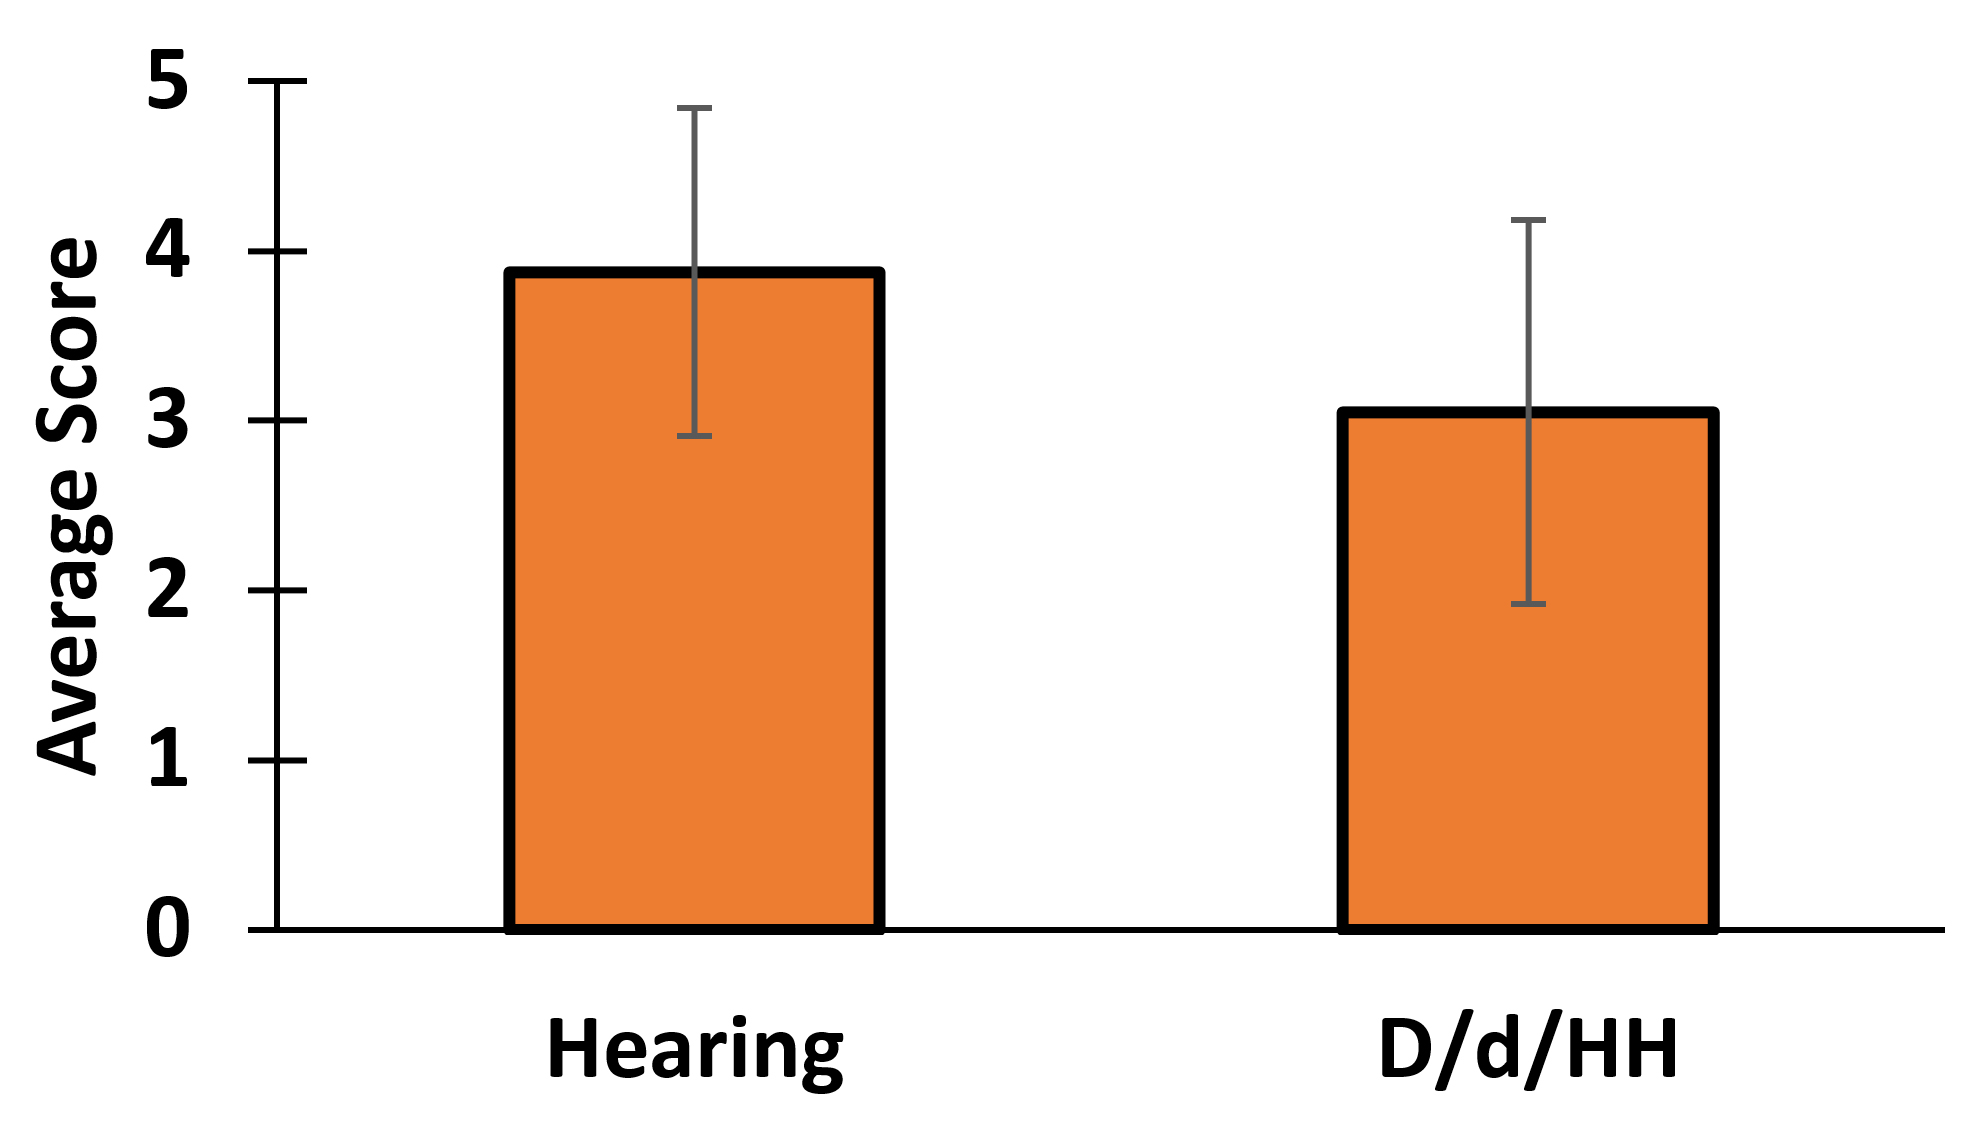
\includegraphics[width=1\linewidth]{Fig1.jpg}
    \caption{Average score/number of correct answers between Hearing and D/d/HH students obtained on the survey.  Error bars represent +/- one standard deviation.}
\end{figure}

The differences may be even more evident as the types of schools that the D/d/HH students attended are expanded. Figure 2 shows the difference between the hearing students and the D/d/HH students separated by whether they attended a “mainstreamed” school or took classes at a residential school for the Deaf.

\begin{figure}[h]
    \centering
    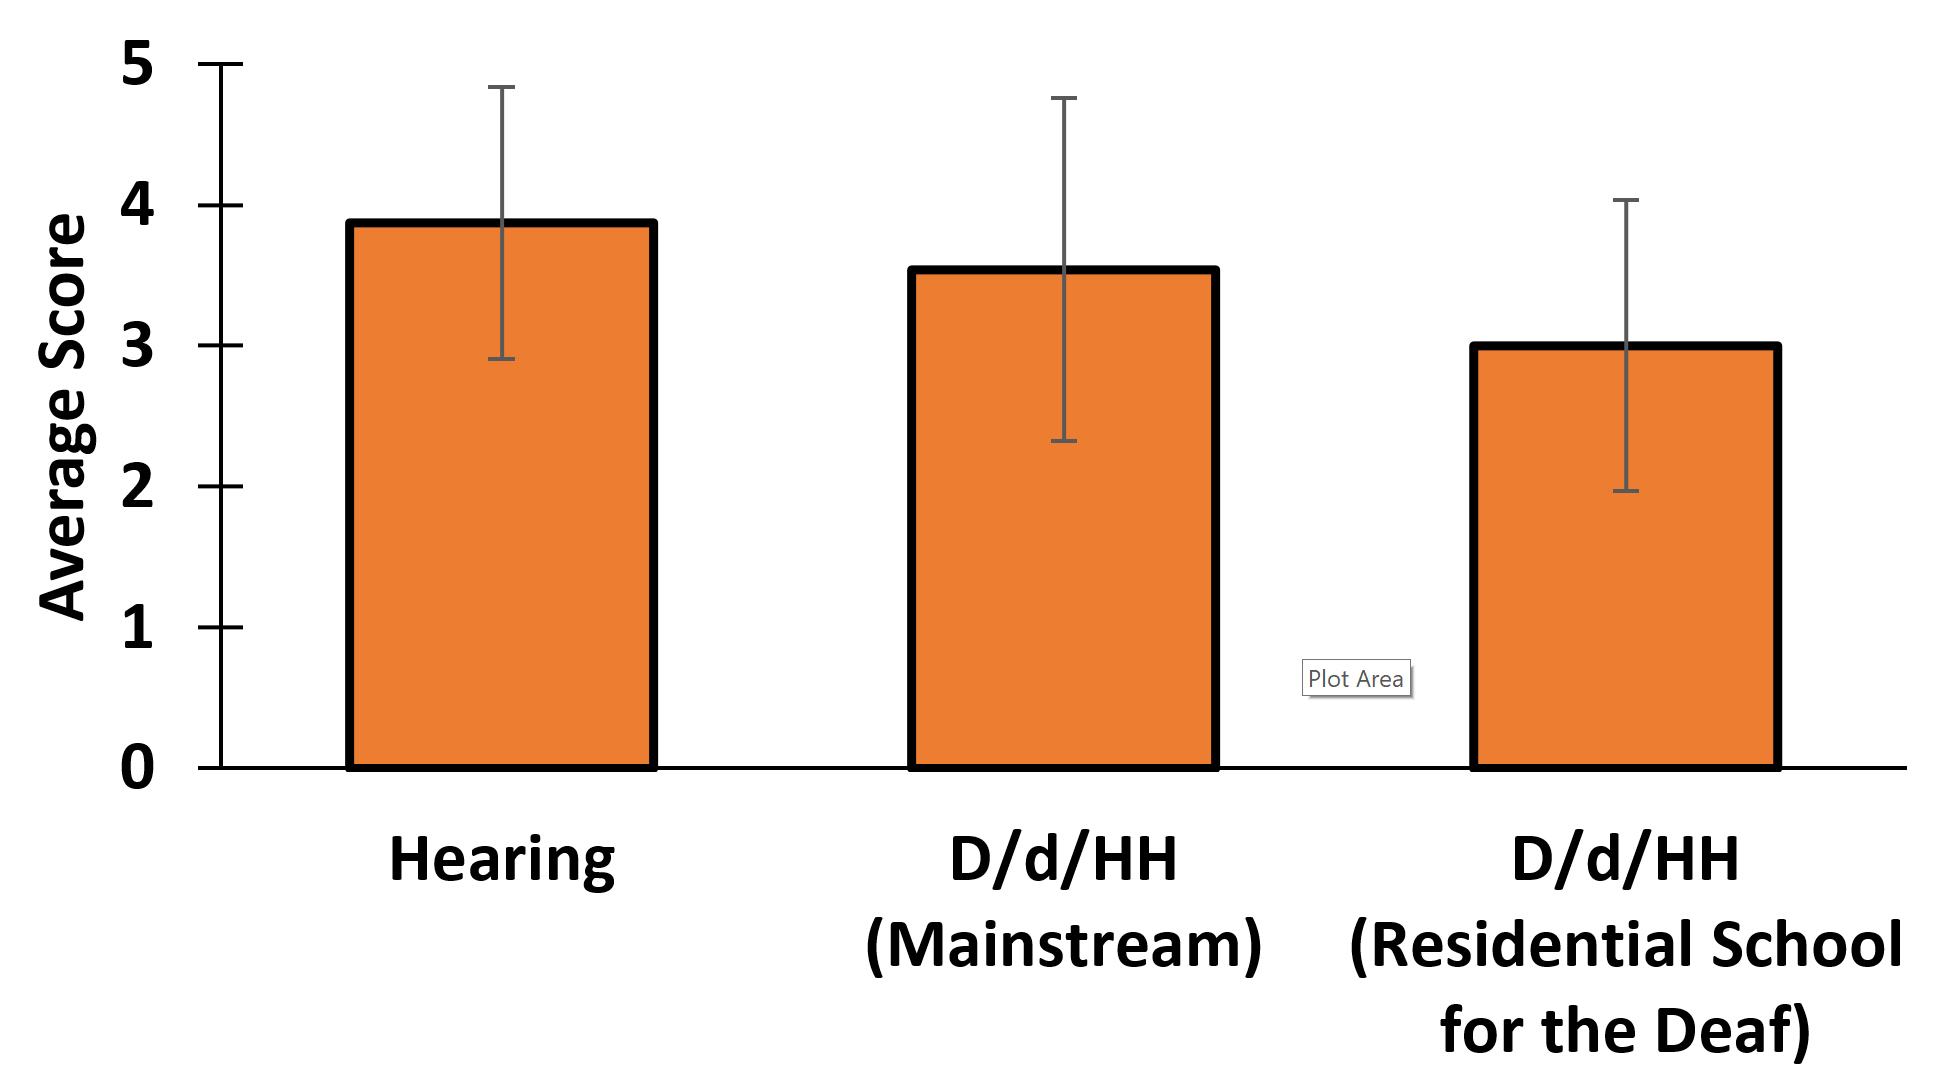
\includegraphics[width=1\linewidth]{Fig2.jpg}
    \caption{Average score/number of correct answers between Hearing and D/d/HH students obtained on the survey, grouped by the type of school they attended.  Error bars represent +/- one standard deviation.}
\end{figure}

In addition to measuring the average score of each student on conceptual questions, we also analyzed the average value that students assigned to themselves based on their perceived knowledge of environmental-related issues (on a 10-point Likert scale). These results are shown in Figure 3.

 \begin{figure}[h]
     \centering
     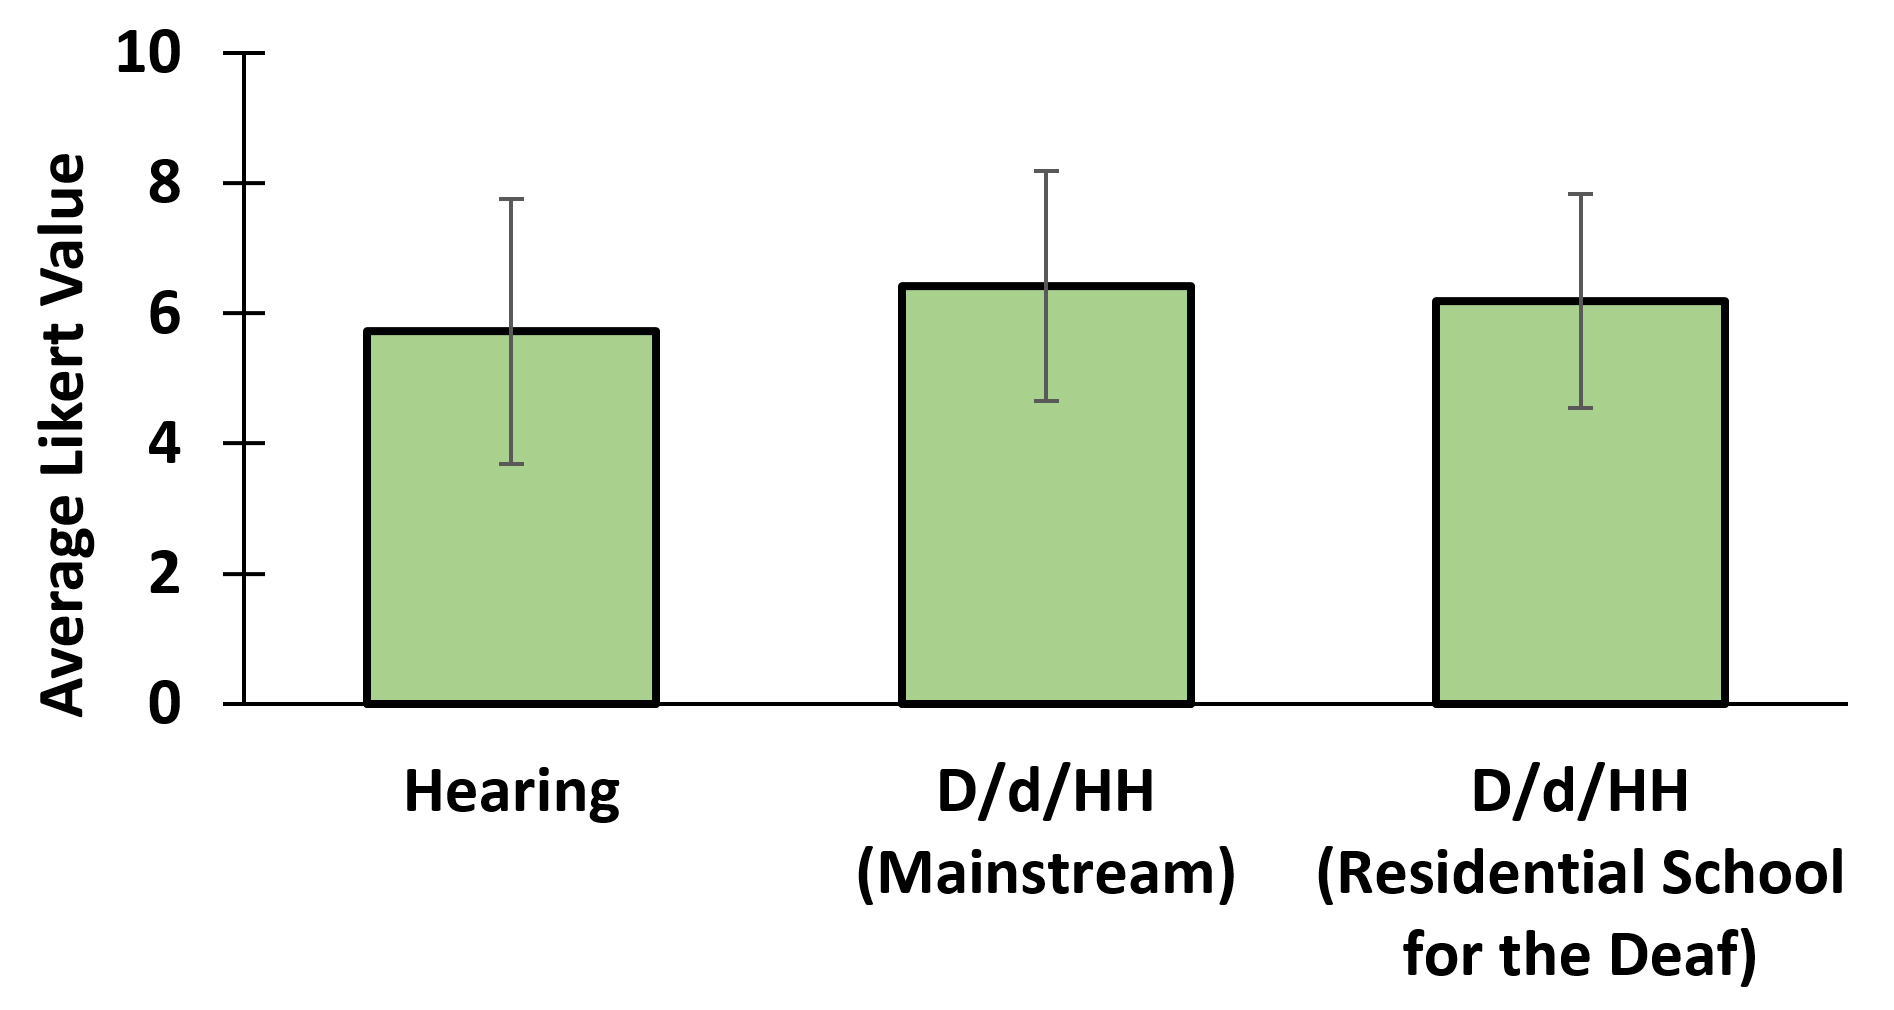
\includegraphics[width=1\linewidth]{Fig3.jpg}
     \caption{Average value from a Likert scale of 1-10 that students chose regarding their perceived knowledge of Environmental Sustainability issues grouped by the type of school they attended.  Error bars represent +/- one standard deviation.}
 \end{figure}

Taking into consideration the students’ perceived knowledge with regards to environmental sustainability, it was also important to understand where they felt they fell on the same Likert scale in regard to how much they believe they can function as a contributing member of society in relation to these environmental issues. These results are shown in Figure 4.
 
\begin{figure}[h]
    \centering
    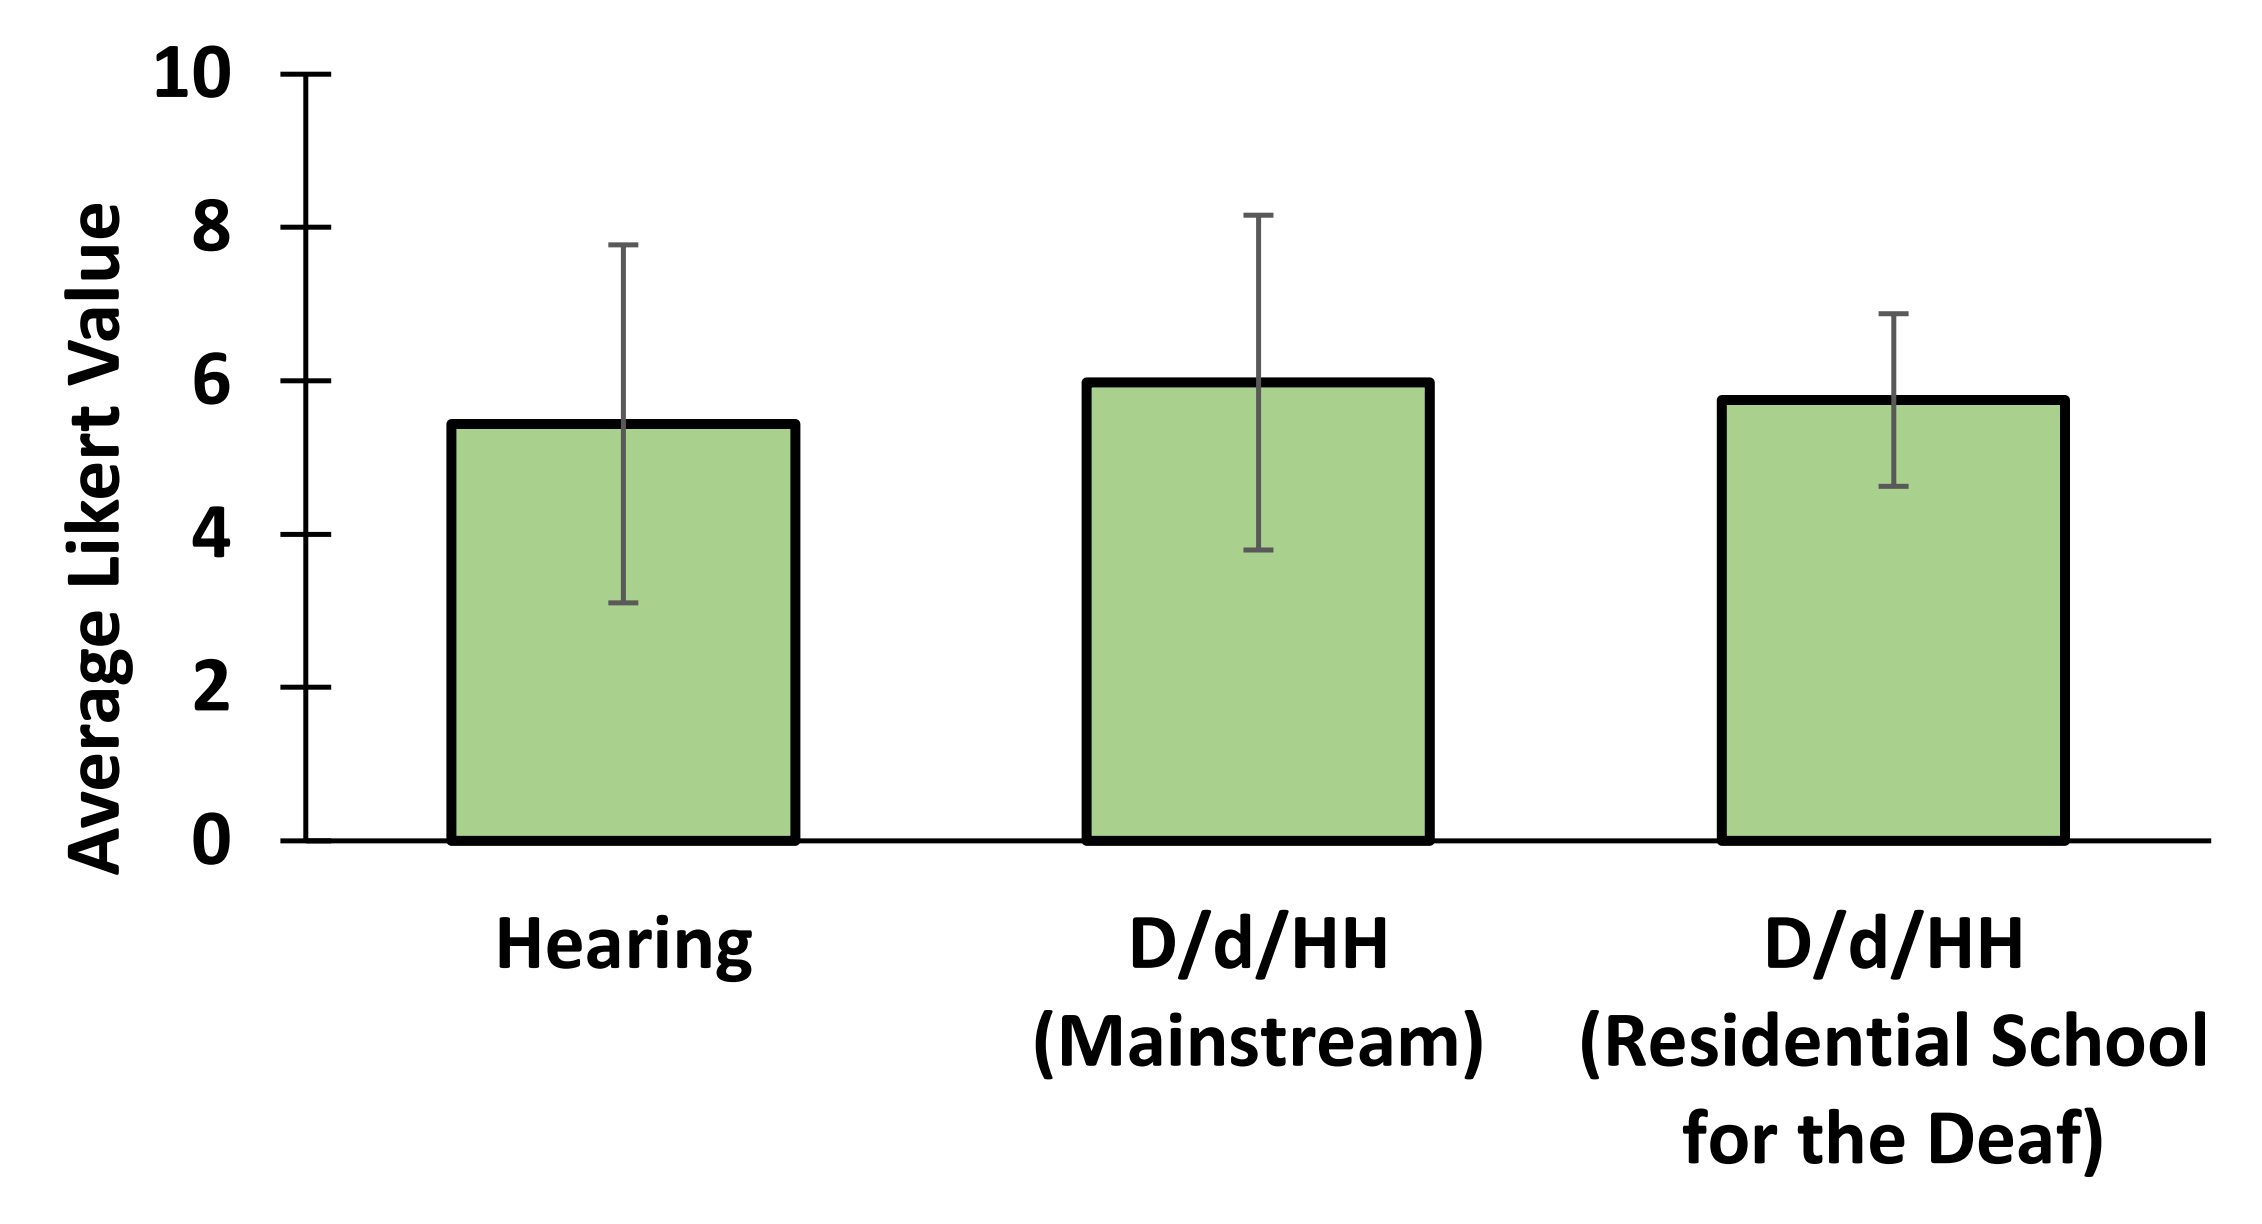
\includegraphics[width=1\linewidth]{Fig4.jpg}
    \caption{Average value from a Likert scale of 1-10 that students chose regarding their perceived ability to function as contributing members of society related to environmental issues, grouped by the type of school they attended.  Error bars represent +/- one standard deviation.}
\end{figure}

The impact of whether a hearing or D/d/HH student would score differently on the instrument is the first piece of desired information if there is truly a gap in how much students understand and learn related to climate science concepts. An analysis of the raw data from the original survey shows that hearing students scored approximately 3.9 correct answers on the survey (out of a total of 5 questions), while the D/d/HH participants scored approximately 3.0 correct answers (Figure 1). In addition, hearing students scored three or higher right answers 36 times compared to 27 times for the D/d/HH students (recall that each of these groups had an equal n=40 participants). This information demonstrates that 67.5\% of the D/d/HH students scored 3 or more correct answers versus 90\% of the hearing students achieving the same benchmark. Further, 12 of the 40 students within the hearing population scored a perfect score, compared to 5 out of the D/d/HH students. Coupled with this raw data, ANOVA analysis revealed a significant difference between hearing and D/d/HH students and their survey scores (F1,78 =  12.31, P = 0.0008). When correcting for the number of High School and College science courses the students had taken, ANCOVA analysis also showed a significant difference (Hearing or D/d/HH:F1,76 =12.08, P = 0.0008; High School science courses: F1,76 = 0.26, P = 0.6130; College science courses: F1,76 = 0.43, P = 0.5148), further demonstrating that hearing participants scored higher than D/d/HH participants.

Participants who identified themselves as D/d/HH were also asked to identify the type of education they received prior to arriving at college. Participants who identified themselves as hearing were instructed not to answer the question regarding the type of school they attended prior to college, as these students would not have attended a residential school for the Deaf. The results show that those participants who did not identify the type of school they attended prior to college scored significantly higher than those who identified themselves as being “mainstreamed” or took classes at residential schools for the Deaf (F2,77=  6.11, P = 0.003;, Figure 2), and the follow-up Tukey HSD test showed that “No answer” (hearing) is significantly higher than “mainstreamed” or residential school for the Deaf. ANCOVA analysis for the same comparison (school type) to take into account the number of high school and college science courses taken by each student found that participants who did not identify the type of school they attended prior to college scored significantly higher than participants who identified themselves as being “mainstreamed” or attending classes at residential schools for the Deaf (School type: F2,75 =6.03, P = 0.0037; High School science courses: F1,76 = 0.29, P = 0.5932; College science courses: F1,76 = 0.48, P = 0.4921). The Tukey HSD follow-up test confirmed that “No answer” (hearing) is significantly higher than “mainstreamed” or “residential school for the Deaf”. 

It is interesting to note that the D/d/HH “mainstreamed” group of participants reported slightly higher, though not statistically significant confidence in perceived knowledge of environmental concepts (F2,77=0.5163,P = 0.67; Figure 3), even though they generally scored lower on the number of correct answers they provided compared to the hearing group. This non-significant pattern was consistent even after correcting for High School science courses and College science courses taken (School type: F2,75 = 0.82, P = 0.4454; High School college courses: F1,75 = 4.64, P = 0.0344; College science courses: F1,75 = 14.78, P = 0.0003).  A more detailed study of whether the language used in the instrument could bias some of the data (as some D/d/HH students have been shown to perform similarly in reading and writing assessments to ELL) was conducted via Rasch analysis. 

\subsection*{Rasch Analysis of the Surveys}

The Rasch analysis of the surveys provides insight as to the language influence regarding the statistically significant difference between D/d/HH students and their hearing peers noted from the original survey.  Throughout the survey assessments, the initial thought was to focus on the quality of the survey as a measurement of conceptual knowledge. However, the phrasing of questions (and multiple-choice options) against levels of students’ English literacy was found to be potentially limiting to the true assessment of conceptual knowledge. Due to the phrasing of certain climate science questions on the initial survey, some D/d/HH students may have been instead tested on their interpretation of the question rather than on their climate science knowledge.  As potentially ELL, some of these students may have been inadvertently tested on a second component: their English mastery. One of the questions in the demographic section of the improved survey asked which English course they were currently taking. The English course represented a DIF analysis of Rasch, and biases against their English literacy were found, largely for True/False questions. 

Throughout the study we completed a total of three iterations of the survey, and in doing so, came to understand how the phrasing and the type of questions might distract from the main goal of assessing climate science knowledge. Future changes that need to be made to the survey include rephrasing multiple-choice questions, and perhaps, the avoidance of using True/False questions altogether. Through the Rasch analysis, we came to understand how the effectiveness of the survey might correspond to student English level.  It is, therefore, important to think about how to phrase the questions so that students at each level of reading/English will be able to understand the content of what is being asked. 
	
 As the first three versions of the surveys were adapted, they were assessed using the Rasch method to measure the quality of the instrument. In summary, there was a lack of unidimensionality in these surveys, as some of the questions required some understanding of other science topics to deduce the correct answer, and as such, the interpretation of the remainder of the survey results should be framed with caution. As previously mentioned, the fact that students may not have interpreted the question correctly also impacts the lack of unidimensionality. In general, the final survey measured at a person reliability of 0.53 and an item reliability of 0.83. Thus, the item reliability is decent while the person reliability was not strong. As a result, closer analysis of the questions and implicit biases is warranted and more changes are needed to improve the survey.

When it came to the item and person-fit of the final survey, the Rasch model performed well. There were some questions that were revised, especially in the choices within the multiple-choice options. A limitation of this latter survey is that the sample population consisted of D/d/HH students beyond LST students, and some of those students did not necessarily have as strong science backgrounds as the LST students (LST students having 1.5 semesters of college science and perhaps being preconditioned to enter STEM fields).  

As the survey was modified, we ascertained that more questions about the participants should be asked to clarify the biases that we had found in the DIF component of the Rasch analysis. The results were unclear as to what specific biases those items implied, so additional demographic questions (mostly related to English level and communication mode/preference were added to the final survey to help identify potential biases. 

While the person reliability was not optimal, there is still value in the final survey since it was the first time we had asked questions regarding student English course level. Using DIF with the final survey version, we found that there were significant differences with some questions in student performance based on their English course level, shown in Table 1. Each color grouping in Table 1 represents the factual question that revealed bias in reference to the students’ reported English/Reading level (correlated English/Reading related background questions asked are shown in column 1).


\begin{table*}[th]
\caption{Questions with Potential Bias Related to English Course or Reading Level on the Final version of the Survey}
\begin{tabular}{|l|l|l|l|l|l|}
\hline
\textbf{English/Reading Level Background Question} & \textbf{Factual Question Type} & \textbf{Those who found the factual question more difficult (biased against)*} & \textbf{Those who found the factual question easier (biased in favor)*} & \textbf{t-stat} & \textbf{p-value} \\ \hline
How would you rate your English reading level? & True/False+ & 1 (Good but need improvement) on a 3-point Likert scale (n=30) & 2 (Very Good) on a 3-point Likert scale & 2.13 & 0.038 \\ \hline
Which English course are you taking now? & True/False+ & Written Communication (NENG-241) (n=10) & Writing Seminar (UWRT-150) (n=19) & 2.56 & 0.0173 \\ \hline
\multirow{2}{=}{Which English course are you taking now?} & \multirow{2}{=}{True/False+} & Bridge to College English II (NENG-232) (n=5) & Written Communication (NENG-241) (n=10) & 2.43 & 0.0381 \\ \hline
 & & Critical Reading and Writing (UWRT-100) (n=7) & Written Communication (NENG-241) (n=10) & 2.92 & 0.0119 \\ \hline
Which English course are you taking now? & Multiple-choice & Critical Reading and Writing (UWRT-100) (n=7) & Writing Seminar (UWRT-150) (n=19) & 2.74 & 0.0151 \\ \hline
\end{tabular}
\\ \\ *Student self-rating or stated enrolled English course. Courses numbered UWRT are generally higher level than those labelled NENG and numbering within each are generally correlated with level. +These questions were also on the original survey.
\end{table*}

Notice in Table 1 that out of the four incidences of questions that showed statistically significant differences between groups, three questions were relevant to the English course in which participants were enrolled, while the fourth instance was related to how the participants assessed their reading levels. Out of the four identified factual survey questions, three were True/False questions. As we continue to improve the survey, we plan to remove these True/False questions and replace them with multiple-choice (or other type) questions, since it seems those questions may be biased related to the students’ literacy abilities. 

As might be expected, all four identified questions showed potential bias against students registered in lower English courses (when compared to groups of students in higher English courses). This type of literacy bias might also be expected of general ELL groups. However, in one instance of a potentially biased question related to English course level, the Rasch analysis identified a second occurrence of bias against a group that was in a higher level English course than the group for which it identified as being potentially biased in favor (Critical Reading and Writing is considered a higher level course than Written Communication in the NTID English course sequence). These two courses, however, are back-to-back/sequential in the English course sequence. Therefore, in cases like this (and with these sample sizes), Rasch may not be able to accurately differentiate English levels of students enrolled in similar level courses. Further, the discrepancy could be due to the fact that the student sample population was not uniform in majors (not all students were science majors- even if in lower English courses, science majors might have the content background to answer the question correctly). As for the remaining multiple-choice question, the multiple-choice frequency table showed that while the correct choice was often chosen by survey participants, the next highest multiple-choice question chosen was phrased very similarly to the correct choice. As a result, the multiple-choice options may warrant rephrasing.

The goal of the survey is not to “penalize” students for literacy challenges (or bias against potential ELL), but rather to measure the amount of knowledge a participant understands regarding climate science. Therefore, English/literacy level of audiences should be taken into consideration when similar assessment tools are developed. And as there is a need for improvement in the quality of measurement tools in education (Bond \& Fox, 2007), the Rasch model provides an accessible method for the development of such instruments.

\section*{CONCLUSION}

Analysis of the original survey showed that hearing participants scored higher on the survey’s factual questions than did their D/d/HH counterparts.  An additional aspect of the survey was related to the participants self-assessment of their knowledge of environmental sustainability issues and their self-assessment of their abilities to function as informed members of society. Lastly, Rasch analyses showed that the phrasing on some questions of the survey might have demonstrated bias against some ASL-primary D/d/HH learners. 

Addressing literacy backgrounds of the students may be important in assuring that the instruments used are indeed sufficient in assessing the climate science knowledge, rather than the participants’ literacy level. In the United States population, students who are primary ASL users is not as large as the group of users of other languages (i.e. Spanish), and therefore, may not be taken into consideration during the development of English-based standardized test/surveys. It is important to recognize that the phrasing of questions on surveys and standardized testing can potentially mislead a unique population, like some D/d/HH students, hence the results from surveys might misrepresent their content knowledge.  However, as the appreciation of assessing the quality of developed surveys/tests grows, more accurate representations of subject-specific content gaps can be revealed, which in turn can lead to more effective interventions. 

Based on this work, we recommend focusing on several main areas in order to improve some of the potential gaps in understanding among some D/d/HH students. First, there is a need to develop more tools for incorporating environmental sustainability and climate science into college science courses.  Importantly, this entails incorporating knowledge about D/d/HH educational needs and environmental education into the current science curriculum. Finally, there is a need for better understanding of language influences regarding D/d/HH and ELL students related to impacts on their learning and demonstration of obtained knowledge.  

\end{large}
\clearpage
\section*{REFERENCES}\par 

\leftskip 0.25in
\parindent -0.25in 
Bond, T. G., \& Fox, C. M. (2007). \textit{Applying the Rasch Model Fundamental Measurement in the Human Sciences} (2nd ed.). New Jersey: Lawrence Erlbaum Associates.

Boone, W. J. (2014). \textit{Rasch Analysis in the Human Sciences}. Retrieved from \url{https://ezproxy.rit.edu/login?url=http://dx.doi.org/10.1007/978-94-007-6857-4}

Chang, C., Pascua, L., \& Ess, F. (2018). Closing the “Hole in the Sky”: The Use of Refutation-Oriented Instruction to Correct Students’ Climate Change Misconceptions. \textit{Journal of Geography, 117}(1), 3–16. \url{https://doi.org/10.1080/00221341.2017.1287768}

Farrington, A. L., Lonigan, C. J., Phillips, B. M., Farver, J. M., \& McDowell, K. D. (2015). Evaluation of the Utility of the “Revised Get Ready to Read!” For Spanish-Speaking English-Language Learners through Differential Item Functioning Analysis. \textit{Assessment for Effective Intervention, 40}(4), 216–227. (SAGE Publications and Hammill Institute on Disabilities. 2455 Teller Road, Thousand Oaks, CA 91320. Tel: 800-818-7243; Tel: 805-499-9774; Fax: 800-583-2665; e-mail: journals@sagepub.com; Web site: \url{http://sagepub.com}).

Gertz, G., \& Boudreault, P. (Eds.). (2016). \textit{The SAGE Deaf Studies Encyclopedia} (Vol. 1–3). Los Angeles: SAGE Publications, Inc.

Guron, M., Paul, J., \& Roeder, M. (2016). Incorporating Sustainability and Life Cycle Assessment into First-Year Inorganic Chemistry Major Laboratories. \textit{Journal of Chemical Education, 93}(4), 639–644. \url{https://doi.org/10.1021/acs.jchemed.5b00281}

Hopper, M. J. (2011). \textit{Positioned as Bystanders: Deaf Students’ Experiences and Perceptions of Informal Learning Phenomena} (Ph.D., University of Rochester). Retrieved from \url{http://search.proquest.com/docview/871882487/abstract/8DD823B150A841B6PQ/12}

King, J. F. (2017, November). Incidental Learning \& the Deaf Child. The Exceptional Parent (Online); Boston, 47(11), 34–35. Retrieved from \url{http://search.proquest.com/docview/1973005318/abstract/8DD823B150A841B6PQ/4}

Lawton, S. B. (2009). \textit{Use and Impact of English-Language Learner Assessment in Arizona}. Online Submission.

Marschark, M. (2001). \textit{Educating deaf students: from research to practice}. Oxford; New York: Oxford University Press.

Marschark, M. (2011). \textit{How deaf children learn: what parents and teachers need to know}. New York: Oxford University Press.

Pagano, T. (2017). Making Education and Careers in Chemistry Accessible and Successful for Deaf and Hard-of-Hearing Students. In Nelson \& Cheng (Series Ed.), \textit{Diversity in the Scientific Community} (pp. 125–132). Washington, D.C.: American Chemical Society.

Pagano, T., Ross, A. D., \& O’Neill, G. J. (2012). A Program Like Any Other-Like None Other: The Laboratory Science Technology Program for Deaf and Hard-of-Hearing Students. \textit{Journal of Science Education for Students with Disabilities, 15}(1), 11–25.

Pagano, T., \& Templeton, D. C. (2018). From Roots to STEM: STEM Education at NTID. In \textit{A Shining Beacon: 50 Years of the National Technical Institute for the Deaf} (pp. 149–160). Rochester, NY: RIT Press.

Rasch, G. (1960). \textit{Probabilistic Models for Some Intelligence and Attainment Tests}. Copenhagen: Danmarks Paedagogiske Institut.

Reckase, M. D., \& Xu, J.-R. (2015). The Evidence for a Subscore Structure in a Test of English Language Competency for English Language Learners. \textit{Educational and Psychological Measurement, 75}(5), 805–825. (SAGE Publications. 2455 Teller Road, Thousand Oaks, CA 91320. Tel: 800-818-7243; Tel: 805-499-9774; Fax: 800-583-2665; e-mail: journals@sagepub.com; Web site: \url{http://sagepub.com}).

Ross, A., Yerrick, R., \& Pagano, T. (2019a). Examining Deaf/Hard-of-Hearing Students’ Equitable Access to Science - An Approach Based on Scientific Argumentation. \textit{Manuscript Submitted for Publication}.

Ross, A., Yerrick, R., \& Pagano, T. (2019b). Examining the use of Argumentation Strategies in Deaf/Hard-of-Hearing Learning Contexts to Teach Climate Science. In \textit{Communication in Chemistry}. Accepted.

Saksiri, B., \& Suphajanya, P. (2010). Global Warming Web-Based Instructional Design for Deaf and Hard-of-Hearing. In D. Gibson \& B. Dodge (Eds.), \textit{Proceedings of Society for Information Technology \& Teacher Education International Conference 2010} (pp. 3755–3758). Retrieved from \url{https://www.learntechlib.org/primary/p/33964/}

Timmer, B. J. J., Schaufelberger, F., Hammarberg, D., Franzen, J., Ramstrom, O., \& Diner, P. (2018). Simple and Effective Integration of Green Chemistry and Sustainability Education into an Existing Organic Chemistry Course. \textit{Journal of Chemical Education, 95}(8), 1301–1306. \url{https://doi.org/10.1021/acs.jchemed.7b00720}

\end{document}